\chapter[主从机时钟对齐]{主从机时钟对齐}[Harbin Institute of Technology Postgraduate Dissertation Writing Specifications]

\section{代码智能提示工具}[Content specification]
在工业自动化和嵌入式系统中,上位机和下位机之间的时间同步是非常重要的。通常,下位机的时间通常是由硬件时钟提供的,
而上位机的时间通常是由操作系统提供的。由于硬件时钟和操作系统时钟存在不同步的可能,因此需要使用网络时间协议(NTP)等工具来同步它们的时间。\par

NTP是一种用于同步计算机时钟的协议,可以通过Internet或局域网等网络连接来实现时钟同步,流程如图\ref{ntp}所示。
NTP通过在网络中分发时间信息来同步时钟,并使用算法来计算不同时钟之间的时间差。使用NTP进行时钟同步时,下位机可以充当NTP客户端,而上位机则可以充当NTP服务器。 \par
\begin{figure}[H]
    \centering
    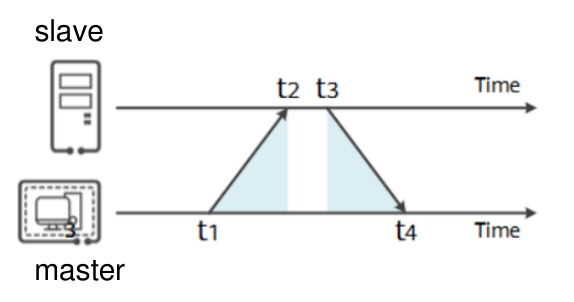
\includegraphics[width=.8\textwidth]{ntp.png} 
    \caption{基于NTP实现时钟同步} 
    \label{ntp}
\end{figure}


使用NTP进行时间同步的优点是它是一种高效、可靠且易于实现的方法。它可以通过网络连接远程同步时钟,并且可以使用各种硬件和操作系统。
然而,由于在下位机中较难安装NTP服务软件,因此本文设计了一个参考NTP方案的基于定频通信的时钟同步系统。\par

基本思想如下:事先通过技术手段测量通信时延。然后以下位机的时钟为基准,下位机定频向上位机发送本机的时钟信息,上位机将计算本机时钟与下位机时钟之差(在考虑通信时延的情况下),
并将数据放入到循环队列中,当需要在上位机获取下位机时钟时刻时,通过计算循环队列的平均值作为offset加到本机时钟就可以获得下位机的时钟时刻,如图\ref{clock_sync}所示。

\begin{figure}[H]
    \centering
    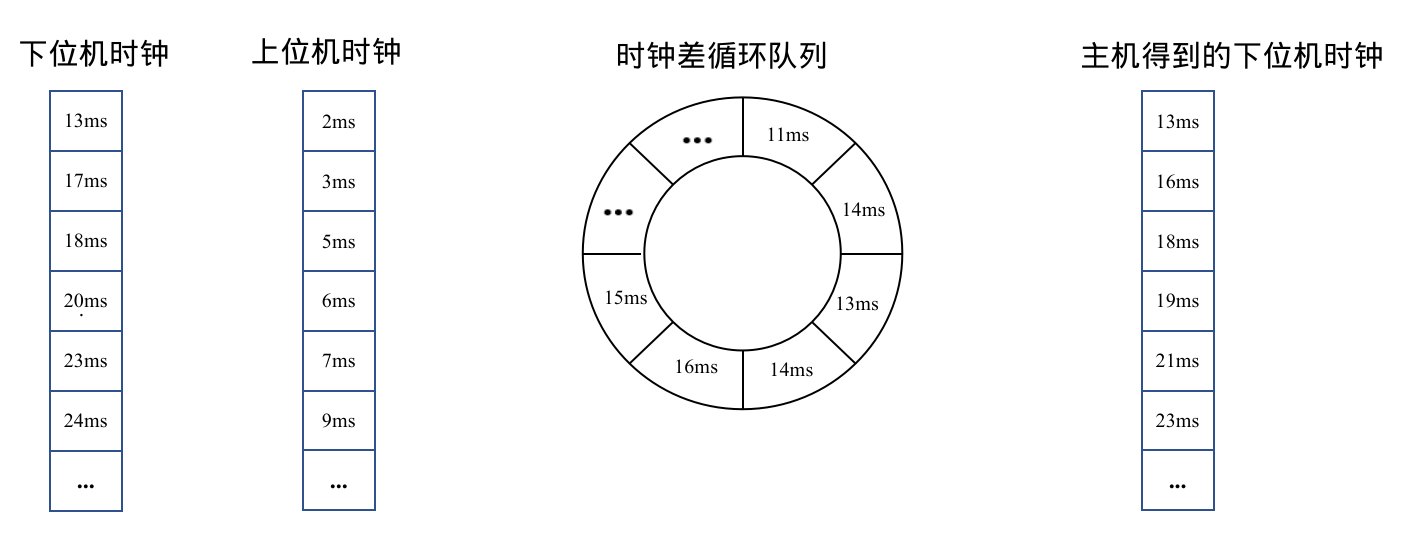
\includegraphics[width=.8\textwidth]{clock_sync.png} 
    \caption{自实现时钟同步} 
    \label{clock_sync}
\end{figure}


\section{通信时延测量}[Content specification]
对于一固定的装甲板,晃动云台,则理论上结算的装甲板在惯性系下的坐标应该是不变的。
然而,由于通信时延、相机成像时间误差、计时精度、陀螺仪数据精度与系统偏差等因素,
不可能精确的获得的图像对应的陀螺仪数据。这里面影响因素最大的就是通信时延,因此通过调节通信时延量,
使得惯性系下的装甲板坐标晃动幅度最后,此时得到的通信时延量认为是真实的通信时延。
\par
图\ref{delay}展示了在通信时延量在超前、滞后、大致准确时解算的装甲板在惯性下的坐标。

\begin{figure}[H]
    \centering
    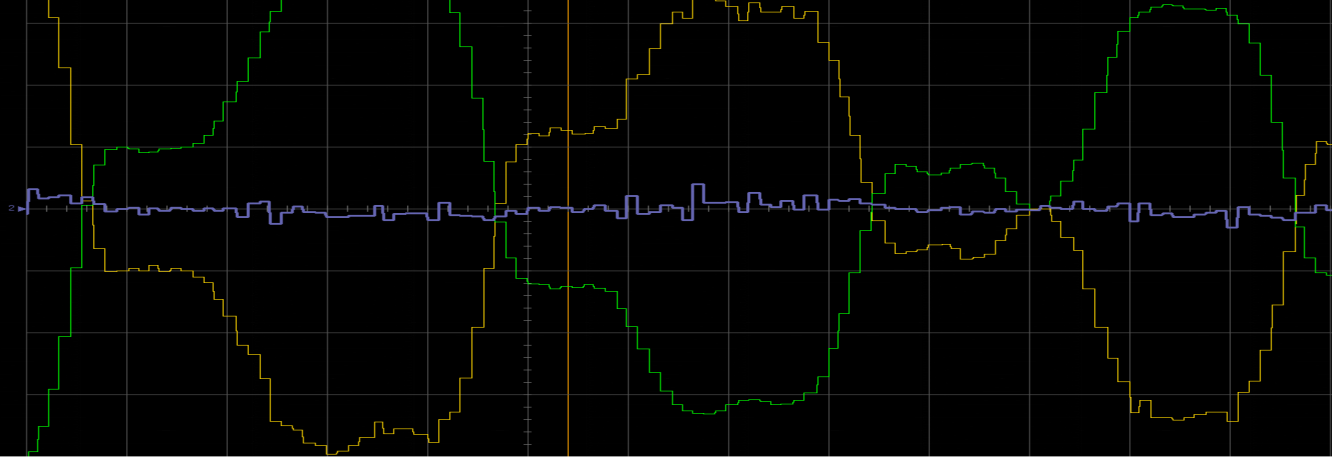
\includegraphics[width=.8\textwidth]{delay.png} 
    \caption{不同通信时延对应的装甲板惯性下的坐标} 
    \label{delay}
\end{figure}




